\documentclass[journal,12pt,onecolumn]{IEEEtran}

\usepackage{amsmath,amssymb,amsfonts,amsthm}

\usepackage{graphicx}

\usepackage{enumitem}

\usepackage[breaklinks=true]{hyperref}

\usepackage{caption}

\usepackage{array}

\newtheorem{problem}{Problem}

\renewcommand{\thefigure}{\theenumi}

\renewcommand{\thetable}{\theenumi}

\usepackage{multicol}

\usepackage{amsmath}

\newcommand{\myvec}[1]{\begin{bmatrix}#1\end{bmatrix}}


\begin{document}

\title{GATE XE 2023}

\author{AI25BTECH11003- Bhavesh Gaikwad}

\maketitle

%------------------------GENERAL APTITUDE------------------

\section*{General Aptitude}

\bigskip

\begin{enumerate}

\item The village was nestled in a green spot, \_\_\_\_\_\_\_ the ocean and the hills.

\hfill{(GATE 2023 XE)}

\begin{multicols}{4}

\begin{enumerate}

\item through

\item in

\item at

\item between

\end{enumerate}

\end{multicols}

\item Disagree : Protest : : Agree : \_\_\_\_\_\_\_  
(By word meaning)

\hfill{(GATE 2023 XE)}

\begin{multicols}{4}

\begin{enumerate}

\item Refuse

\item Pretext

\item Recommend

\item Refute

\end{enumerate}

\end{multicols}

\item A ‘frabjous’ number is defined as a 3 digit number with all digits odd, and no two 
adjacent digits being the same. For example, 137 is a frabjous number, while 133 
is not. How many such frabjous numbers exist?

\hfill{(GATE 2023 XE)}

\begin{multicols}{4}

\begin{enumerate}

\item 125

\item 720

\item 60

\item 80

\end{enumerate}

\end{multicols}

\item Which one among the following statements must be TRUE about the mean and 
the  median of the scores of all candidates appearing for GATE 2023?

\hfill{(GATE 2023 XE)}

\begin{multicols}{2}

\begin{enumerate}

\item The median is at least as large as the mean.

\item The mean is at least as large as the median.

\item At most half the candidates have a score that is larger than the median.

\item At most half the candidates have a score that is larger than the mean.

\end{enumerate}

\end{multicols}


\item In the given diagram, ovals are marked at different heights (h) of a hill. Which one 
of the following options P, Q, R, and S depicts the top view of the hill?

\begin{figure}[htbp]

\centering

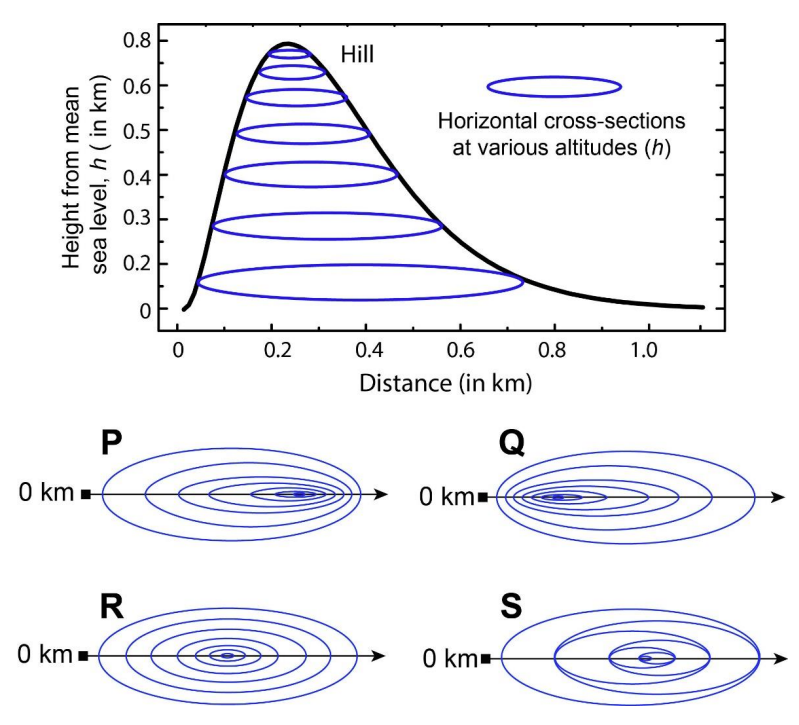
\includegraphics[width=.2\columnwidth]{figs/GA/fig1.png}

\caption{Diagram}

\label{fig:figs/GA/fig1.png}

\end{figure}

\hfill{(GATE 2023 XE)}

\begin{multicols}{4}

\begin{enumerate}

\item P

\item Q

\item R

\item S

\end{enumerate}

\end{multicols}


\newpage

\item Residency is a famous housing complex with many well-established individuals 
among its residents. A recent survey conducted among the residents of the 
complex revealed that all of those residents who are well established in their 
respective fields happen to be academicians. The survey also revealed that most of 
these academicians are authors of some best-selling books. 
 
Based only on the information provided above, which one of the following 
statements can be logically inferred with certainty?

\hfill{(GATE 2023 XE)}

\begin{multicols}{2}

\begin{enumerate}

\item Some residents of the complex who are well established in their fields are also 
authors of some best-selling books.

\item All academicians residing in the complex are well established in their fields.

\item Some authors of best-selling books are residents of the complex who are well 
established in their fields.

\item Some academicians residing in the complex are well established in their fields.

\end{enumerate}

\end{multicols}

\item Ankita has to climb 5 stairs starting at the ground, while respecting the following 
rules: 
1. At any stage, Ankita can move either one or two stairs up. 
2. At any stage, Ankita cannot move to a lower step. 
Let F(n) denote the number of possible ways in which Ankita can reach the Nth  stair. For example, F(1) = 1, F(2) =  2, F(3) =  3. 
The value of F(5) is \_\_\_\_\_\_\_.

\hfill{(GATE 2023 XE)}

\begin{multicols}{4}

\begin{enumerate}

\item 8

\item 7

\item 6

\item 5

\end{enumerate}

\end{multicols}

\item The information contained in DNA is used to synthesize proteins that are 
necessary for the functioning of life. DNA is composed of four nucleotides: 
Adenine (A), Thymine (T), Cytosine (C), and Guanine (G). The information 
contained in DNA can then be thought of as a sequence of these four nucleotides: 
A, T, C, and G. DNA has coding and non-coding regions. Coding regions—where 
the sequence of these nucleotides are read in groups of three to produce individual 
amino  
acids—constitute only about 2\% of human DNA. For example, the triplet of 
nucleotides CCG codes for the amino acid glycine, while the triplet GGA codes 
for the amino acid proline. Multiple amino acids are then assembled to form a 
protein.  
Based only on the information provided above, which of the following statements 
can be logically inferred with certainty? 
(i) 
The majority of human DNA has no role in the synthesis of proteins. 
(ii) 
The function of about 98\% of human DNA is not understood.

\hfill{(GATE 2023 XE)}

\begin{multicols}{2}

\begin{enumerate}

\item only (i)

\item only (ii)

\item both (i) and (ii)

\item neither (i) nor (ii)

\end{enumerate}

\end{multicols}

\newpage
\item Which one of the given figures P, Q, R and S represents the graph of the following $f(x) = ||x+2| - |x-1||$ function? 


\begin{figure}[htbp]

\centering

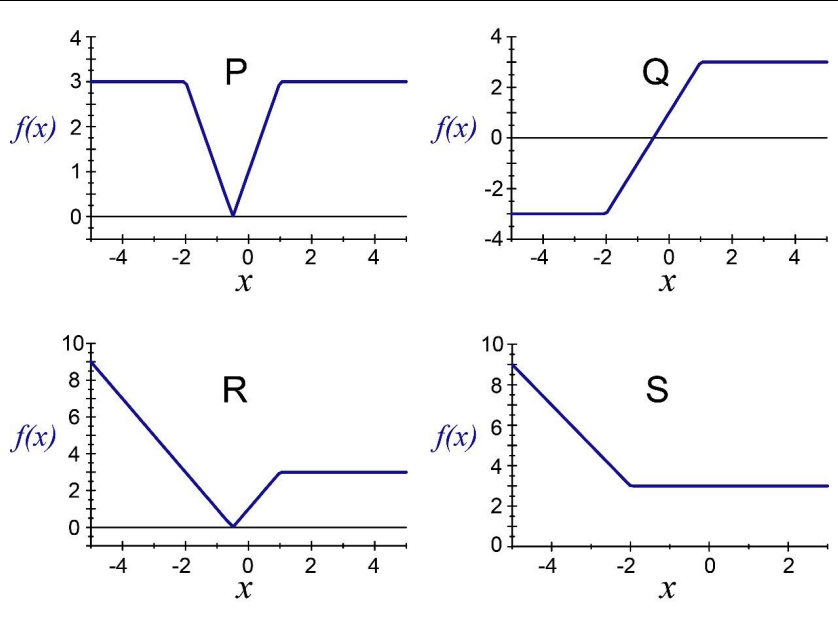
\includegraphics[width=.4\columnwidth]{figs/GA/fig2.png}

\caption{(Graphs)}

\label{fig:figs/GA/fig2.png}

\end{figure}

\hfill{(GATE 2023 XE)}

\begin{multicols}{4}

\begin{enumerate}

\item P

\item Q

\item R

\item S

\end{enumerate}

\end{multicols}



\item An opaque cylinder (shown below) is suspended in the path of a parallel beam of 
light, such that its shadow is cast on a screen oriented perpendicular to the 
direction of the light beam. The cylinder can be reoriented in any direction within 
the light beam. Under these conditions, which one of the shadows P, Q, R, and S 
is NOT possible?

\begin{figure}[htbp]

\centering

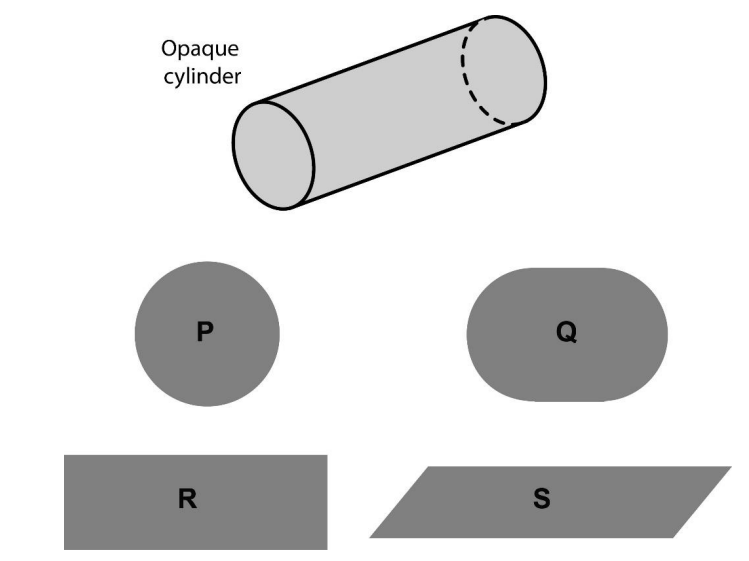
\includegraphics[width=.4\columnwidth]{figs/GA/fig3.png}

\caption{Cylinder and Its Shadows}

\label{fig:figs/GA/fig3.png}

\end{figure}

\hfill{(GATE 2023 XE)}

\begin{multicols}{4}

\begin{enumerate}

\item P

\item Q

\item R

\item S

\end{enumerate}

\end{multicols}

\end{enumerate}

\begin{center}

\item[\textbf{END OF SECTION- GA}]

\end{center}

%---------------------SECTION-A---------------
\newpage
\section*{Engineering Mathematics}

\noindent

\bigskip

\begin{enumerate}

\item Let $A$ be a $3 \times 3$ real matrix having eigenvalues 1, 2, and 3. If $B= A^2 + 2A + I$,
where $I$ is the $3 \times 3$ identity matrix, then the eigenvalues of $B$ are

\hfill{(GATE 2023 XE)}

\begin{multicols}{2}

\begin{enumerate}

\item 4, 9, 16

\item 1, 2, 3

\item 1, 4, 9

\item 4, 16, 25

\end{enumerate}

\end{multicols}

\item Let $f: \mathbb{R}^2 \to \mathbb{R}$ be a function defined by
$f(x,y)=
\begin{cases}
\dfrac{x,y}{|x|+y} & \text{if } y\neq -|x| \\
0 , & \text{otherwise}
\end{cases}$

Then which one of the following statement is TRUE?

\hfill{(GATE 2023 XE)}

\begin{multicols}{2}

\begin{enumerate}

\item $f$ is NOT continuous at $(0,0)$.

\item $\frac{\partial f}{\partial x}(0,0) = 0$, and $\frac{\partial f}{\partial y}(0,0) = 1$.

\item $\frac{\partial f}{\partial x}(0,0) = 1$, and $\frac{\partial f}{\partial y}(0,0) = 0$.

\item $\frac{\partial f}{\partial x}(0,0) = 1$, and $\frac{\partial f}{\partial y}(0,0) = 1$.

\end{enumerate}

\end{multicols}

\item If the quadrature formula

$\int_{-1}^1 f(x) dx \approx \frac{1}{9}\left(c_1 f(-1) + c_2 f(\frac{1}{2}) + c_3 f(1)\right)$

is exact for all polynomials of degree less than or equal to 2, then

\hfill{(GATE 2023 XE)}

\begin{multicols}{2}

\begin{enumerate}

\item $c_1 + \frac{c_2}{4} + c_3 = 6$

\item $c_1 + \frac{c_2}{3} + c_3 = 4$

\item $c_1 + \frac{c_2}{2} + c_3 = 2$

\item $c_1 + c_2 + c_3 = 5$

\end{enumerate}

\end{multicols}

\item The second smallest eigenvalue of the eigenvalue problem

$\frac{d^2 y}{d x^2} + (\lambda - 3) y = 0$, $y(0) = y(\pi) = 0$,

is

\hfill{(GATE 2023 XE)}

\begin{multicols}{2}

\begin{enumerate}

\item 4

\item 3

\item 7

\item 9

\end{enumerate}

\end{multicols}

\item Which one of the following functions is differentiable at $z=0$ but NOT
differentiable at any other point in the complex plane $\mathbb{C}$?

\hfill{(GATE 2023 XE)}

\begin{multicols}{2}

\begin{enumerate}

\item $f(z) = z |z|$, $z \in \mathbb{C}$

\item $f(z) = \sin(z)$, $z \in \mathbb{C}$

\item $f(z)=
         \begin{cases}
       e^{1/z} & , z\neq 0,\\
         0 & , z=0
        \end{cases}$

\item $f(z) = e^{-z^2}$, $z \in \mathbb{C}$

\end{enumerate}

\end{multicols}

\item If the polynomial

$P(x) = a_0 + a_1 x + a_2 x(x-1) + a_3 x(x-1)(x-2)$

interpolates the points $(0,2), (1,3), (2,2)$ and $(3,5)$, then the value of $P(\frac{5}{2})$ is \underline{\hspace{3cm}} (round off to 2 decimal places).

\hfill{(GATE 2023 XE)}

\newpage

\item The value of $m$ for which the vector field

$\vec{F}(x,y) = (4x^m y^2 - 2 x y^m) \hat{i} + (2 x^4 y - 3 x^2 y^2) \hat{j}$

is a conservative vector field, is \_\_\_\_\_\_\_\_\_ (integer).

\hfill{(GATE 2023 XE)}

\item Let  $P = \myvec{4 & -2 & 2\\ 6 & -3 & 4\\ 3 & -2 & 3}$ and $Q = \myvec{3 & -2 & 2\\ 4 & -4 & 6\\ 2 & -3 & 5}$.\\

The eigenvalues of both $P$ and $Q$ are $1, 1, 2$. Which one of the following
statements is TRUE?

\hfill{(GATE 2023 XE)}

\begin{multicols}{2}

\begin{enumerate}

\item Both $P$ and $Q$ are diagonalizable

\item $P$ is diagonalizable but $Q$ is NOT diagonalizable

\item $P$ is NOT diagonalizable but $Q$ is diagonalizable

\item Both $P$ and $Q$ are NOT diagonalizable

\end{enumerate}

\end{multicols}

\item The surface area of the portion of the paraboloid

$z = x^2 + y^2$

that lies between the planes $z=0$ and $z=1/4$ is

\hfill{(GATE 2023 XE)}

\begin{multicols}{2}

\begin{enumerate}

\item $\frac{\pi}{6} (2\sqrt{2} -1)$

\item $\frac{\pi}{2} (2\sqrt{2} -1)$

\item $\pi (2\sqrt{2} -1)$

\item $\frac{\pi}{3} (2\sqrt{2} -1)$

\end{enumerate}

\end{multicols}

\item The probability of a person telling the truth is $\frac{4}{6}$. An unbiased die is thrown twice by
the same person and the person reports that the numbers appeared in both
throws are same. Then the probability that actually the numbers appeared in
both throws are same is \_\_\_\_\_\_\_ (round off to 2 decimal places).

\hfill{(GATE 2023 XE)}

\item Let $u(x,t)$ be the solution of the initial boundary value problem

$\frac{\partial u}{\partial t} - \frac{\partial^2 u}{\partial x^2} = 0$, for $x , \in , (0,2), t > 0$ with initial condition $u(x,0) = \sin (\pi x)$ for $x , \in , (0,2)$ and boundary conditions $u(0,t) = u(2,t) = 0$

Then the value of $e^{\pi^2} (u(\frac{1}{2},1) - u(\frac{3}{2},1))$ is \_\_\_\_\_\_\_ (integer).

\hfill{(GATE 2023 XE)}

\end{enumerate}

\begin{center}

\item[\textbf{END OF SECTION-A}]

\end{center}


\newpage
%---------------------SECTION-B---------------

\section*{Fluid Mechanics}
\bigskip

\begin{enumerate}

% Q1 
\item Match the following measuring instruments with the appropriate figures.\\
I – Pitot probe \quad II – Pitot-static probe \quad III – Piezometer

\begin{figure}[htbp]
\centering
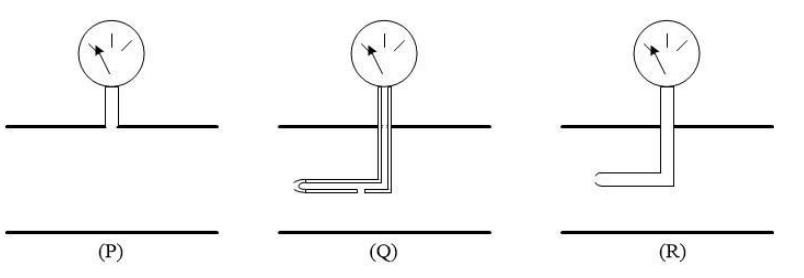
\includegraphics[width=0.8\columnwidth]{figs/B/fig1.png}
\caption{Figures for matching instruments}
\label{fig:figs/Bfig1.png}
\end{figure}
\hfill{(GATE 2023 XE)}

\begin{multicols}{2}
\begin{enumerate}
\item I – P; II – Q; III – R
\item I – R; II – Q; III – P
\item I – R; II – P; III – Q
\item I – Q; II – P; III – R
\end{enumerate}
\end{multicols}

% Q2 
\item Among the following non-dimensional numbers, which one characterizes periodicity
present in a transient flow?
\hfill{(GATE 2023 XE)}
\begin{multicols}{2}
\begin{enumerate}
\item Froude number
\item Strouhal number
\item Peclet number
\item Lewis number
\end{enumerate}
\end{multicols}

% Q3 
\item For an incompressible boundary layer flow over a flat plate shown in the figure, the
momentum thickness is expressed as

\begin{figure}[htbp]
\centering
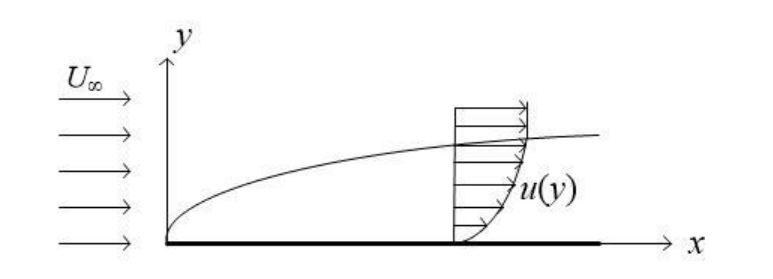
\includegraphics[width=0.7\columnwidth]{figs/B/fig2.png}
\caption{Flat plate boundary layer schematic}
\label{fig:figs/B/fig2.png}
\end{figure}
\hfill{(GATE 2023 XE)}
\begin{multicols}{2}
\begin{enumerate}
\item $\displaystyle \int_0^{\infty}\frac{u}{U_\infty}\,dy$
\item $\displaystyle \int_0^{\infty}\left(1-\frac{u}{U_\infty}\right)\,dy$
\item $\displaystyle \int_0^{\infty}\frac{u}{U_\infty}\left(1-\frac{u}{U_\infty}\right)\,dy$
\item $\displaystyle \int_0^{\infty}\left(1-\frac{u^2}{U_\infty^2}\right)\,dy$
\end{enumerate}
\end{multicols}

\newpage

% Q4 
\item Among the shear stress versus shear strain rate curves shown in the figure, which one
corresponds to a shear thinning fluid?

\begin{figure}[htbp]
\centering
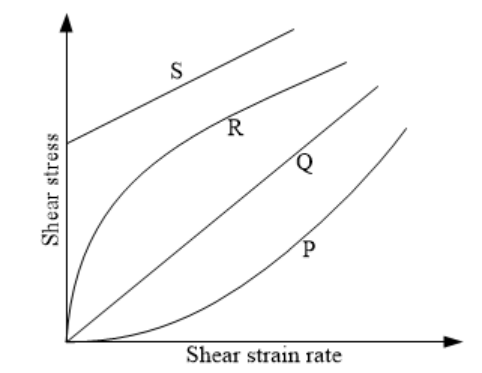
\includegraphics[width=0.7\columnwidth]{figs/B/fig3.png}
\caption{Shear stress vs. shear rate curves}
\label{fig:figs/B/fig3.png}
\end{figure}
\hfill{(GATE 2023 XE)}
\begin{multicols}{2}
\begin{enumerate}
\item P
\item Q
\item R
\item S
\end{enumerate}
\end{multicols}

% Q5 
\item Consider steady incompressible flow over a flat plate, where the dashed line
represents the edge of the boundary layer, as shown in the figure. Which one among
the following statements is true?

\begin{figure}[htbp]
\centering
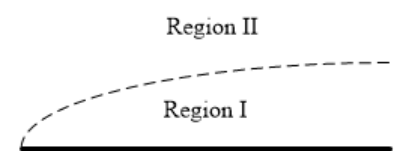
\includegraphics[width=0.75\columnwidth]{figs/B/fig4.png}
\caption{Regions relative to boundary layer}
\label{fig:figs/B/fig4.png}
\end{figure}
\hfill{(GATE 2023 XE)}
\begin{multicols}{2}
\begin{enumerate}
\item Bernoulli’s equation can be applied in Region I between any two arbitrary points.
\item Bernoulli’s equation can be applied in Region I only along a streamline.
\item Bernoulli’s equation cannot be applied in Region II.
\item Bernoulli’s equation cannot be applied in Region I.
\end{enumerate}
\end{multicols}

% Q6
\item An inviscid steady incompressible flow is formed by combining a uniform flow with
velocity $U_\infty$ and a clockwise vortex of strength $K$ at the origin, as shown in the
figure. Velocity potential ($\phi$) for the combined flow in polar coordinate $(r,\theta)$ is

\begin{figure}[htbp]
\centering
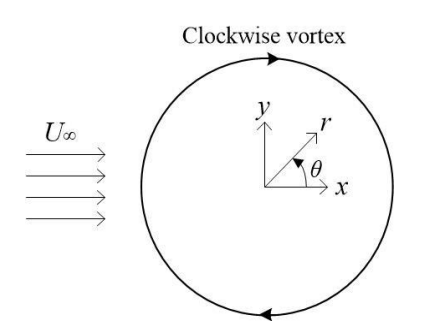
\includegraphics[width=0.6\columnwidth]{figs/B/fig5.png}
\caption{Uniform flow plus vortex}
\label{figfigs/B/fig5.png}
\end{figure}
\hfill{(GATE 2023 XE)}
\begin{multicols}{2}
\begin{enumerate}
\item $\phi=\dfrac{K\theta}{2\pi}-U_\infty r\cos\theta$
\item $\phi=\dfrac{K\theta}{2\pi}-U_\infty r\sin\theta$
\item $\phi=K\ln r+U_\infty r\cos\theta$
\item $\phi=-K\ln r+U_\infty r\sin\theta$
\end{enumerate}
\end{multicols}

% Q7 
\item Which of the following statements are true?\\
(i) Conservation of mass for an unsteady incompressible flow can be represented as
$\nabla\cdot \vec{V}=0$, where $\vec{V}$ denotes velocity vector.\\
(ii) Circulation is defined as the line integral of vorticity about a closed curve.\\
(iii) For some fluids, shear stress can be a nonlinear function of the shear strain rate.\\
(iv) Integration of the Bernoulli’s equation along a streamline under steady-state
leads to the Euler’s equation.
\hfill{(GATE 2023 XE)}
\begin{multicols}{2}
\begin{enumerate}
\item (i), (ii) and (iv) only
\item (i), (ii) and (iii) only
\item (i) and (iii) only
\item (ii) and (iv) only
\end{enumerate}
\end{multicols}

\newpage

% Q8 
\item For a two-dimensional flow field given as $\vec{V}= -x\,\hat{i} + y\,\hat{j}$, a streamline passes
through points $(2,1)$ and $(5,p)$. The value of $p$ is
\hfill{(GATE 2023 XE)}
\begin{multicols}{2}
\begin{enumerate}
\item 5
\item $5/2$
\item $2/5$
\item 2
\end{enumerate}
\end{multicols}


% Q9 
\item A stationary object is fully submerged in a static fluid, as shown in the figure. Here,
CG and CB stand for center of gravity and center of buoyancy, respectively. Which
one(s) among the following statements is/are true?
\hfill{(GATE 2023 XE)}
\begin{figure}[htbp]
\centering
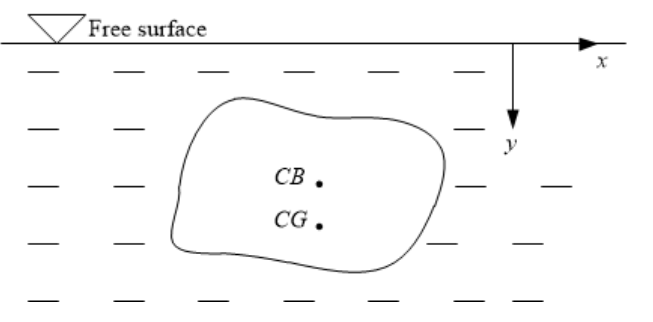
\includegraphics[width=0.7\columnwidth]{figs/B/fig6.png}
\caption{Submerged object with CG and CB}
\label{fig:figs/B/fig6.png}
\end{figure}

\begin{multicols}{2}
\begin{enumerate}
\item The object is in stable equilibrium if $y_{CG}>y_{CB}$.
\item The object is in stable equilibrium if $y_{CG}<y_{CB}$.
\item The object is in neutral equilibrium if $y_{CG}=y_{CB}$.
\item The object is in unstable equilibrium if $y_{CG}=y_{CB}$.
\end{enumerate}
\end{multicols}

% Q10
\item Consider steady fully-developed incompressible flow of a Newtonian fluid
between two infinite parallel flat plates. The plates move in the opposite
directions, as shown in the figure. In the absence of body force and pressure
gradient, the ratio of shear stress at the top surface $(y=H)$ to that at the bottom
surface $(y=0)$ is

\begin{figure}[htbp]
\centering
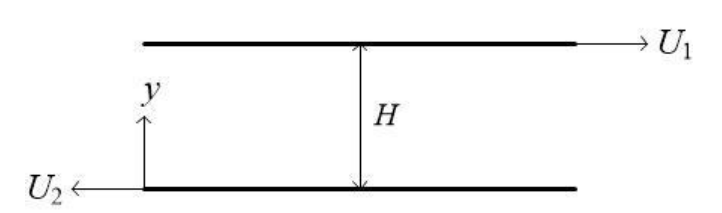
\includegraphics[width=0.75\columnwidth]{figs/B/fig7.png}
\caption{Couette flow between plates}
\label{fig:figs/B/fig7.png}
\end{figure}
\hfill{(GATE 2023 XE)}
\begin{multicols}{2}
\begin{enumerate}
\item 1
\item $U_1/U_2$
\item $(U_1-U_2)/U_2$
\item $(U_1+U_2)/U_2$
\end{enumerate}
\end{multicols}

% Q11 
\item A two-dimensional incompressible flow field is defined as, 
$\vec{V}(x,y)=(Axy)\,\hat{i}+(By^2)\,\hat{j}$ where, $A$ and $B$ are constants. The dynamic
viscosity of the Newtonian fluid is $\mu$. In the absence of body force, which among
the following expressions represents the pressure gradient at the location $(5,0)$ in
the concerned flow field?
\hfill{(GATE 2023 XE)}
\begin{multicols}{2}
\begin{enumerate}
\item $\mu A(5\,\hat{i}+\hat{j})$
\item $\mu(-5B\,\hat{i}+A\,\hat{j})$
\item $\mu A(-\hat{j})$
\item $\mu A(5\,\hat{i})$
\end{enumerate}
\end{multicols}

% Q12 
\item For a potential flow, the fluid velocity is given by $\vec{V}(x,y)=u\,\hat{i}+v\,\hat{j}$. The slope
of the potential line at $(x,y)$ is
\hfill{(GATE 2023 XE)}
\begin{multicols}{2}
\begin{enumerate}
\item $u/v$
\item $v/u$
\item $-u/v$
\item $-v/u$
\end{enumerate}
\end{multicols}

% Q13
\item Consider steady incompressible flow of a Newtonian fluid over a horizontal flat
plate, as shown in the figure. The boundary layer thickness is proportional to

\begin{figure}[htbp]
\centering
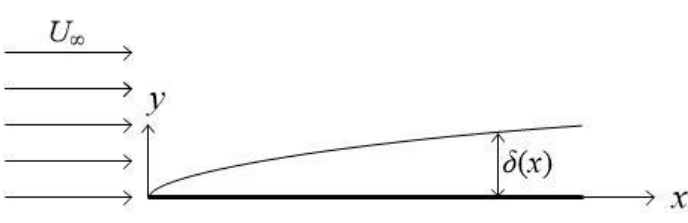
\includegraphics[width=0.7\columnwidth]{figs/B/fig8.png}
\caption{Flat plate boundary layer growth}
\label{fig:figs/B/fig8.png}
\end{figure}
\hfill{(GATE 2023 XE)}
\begin{multicols}{2}
\begin{enumerate}
\item $x^{1/4}$
\item $x^{1/2}$
\item $x^{-1/2}$
\item $x^2$
\end{enumerate}
\end{multicols}

% Q14
\item In a steady two-dimensional compressible flow, $u$ and $v$ are the $x$- and $y$-
components of flow velocity, respectively and $\rho$ is the fluid density. Among the
following pairs of relations, which one(s) perfectly satisfies/satisfy the definition
of stream function, $\psi$, for this flow?
\hfill{(GATE 2023 XE)}
\begin{multicols}{2}
\begin{enumerate}
\item $u=\dfrac{\partial \psi}{\partial y}$ and $v=-\dfrac{\partial \psi}{\partial x}$
\item $u=-\dfrac{\partial \psi}{\partial x}$ and $v=-\dfrac{\partial \psi}{\partial y}$
\item $\rho u=\dfrac{\partial \psi}{\partial y}$ and $\rho v=-\dfrac{\partial \psi}{\partial x}$
\item $\rho u=-\dfrac{\partial \psi}{\partial y}$ and $\rho v=\dfrac{\partial \psi}{\partial x}$
\end{enumerate}
\end{multicols}

\newpage

% Q15
\item A water jet (density = 1000 kg/m$^3$) is approaching a vertical plate, having an
orifice at the center, as shown in the figure. While a part of the jet passes through
the orifice, remainder flows along the plate. Neglect friction and assume both the
inlet and exit jets to have circular cross-sections. If $V=5$ m/s, $D=100$ mm and
$d=25$ mm, magnitude of the horizontal force (in N, rounded off to one decimal
place) required to hold the plate in its position is \_\_\_\_\_\_.

\begin{figure}[htbp]
\centering
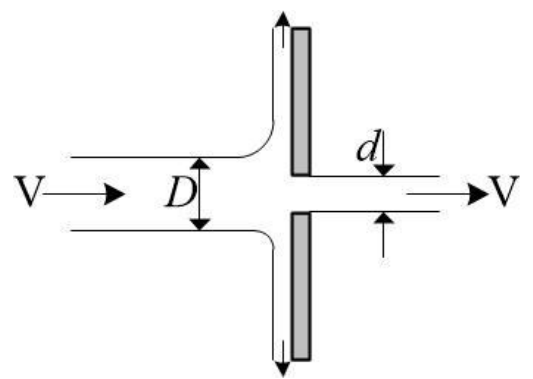
\includegraphics[width=0.4\columnwidth]{figs/B/fig9.png}
\caption{Jet impacting perforated plate}
\label{fig:figs/B/fig9.png}
\end{figure}
\hfill{(GATE 2023 XE)}

% Q16
\item Water (density = 1000 kg/m$^3$) and alcohol (specific gravity = 0.7) enter a
Y-shaped channel at flow rates of 0.2 m$^3$/s and 0.3 m$^3$/s, respectively. Their
mixture leaves through the other end of the channel, as shown in the figure. The
average density (in kg/m$^3$) of the mixture is \_\_\_\_\_\_\_\_\_.

\begin{figure}[htbp]
\centering
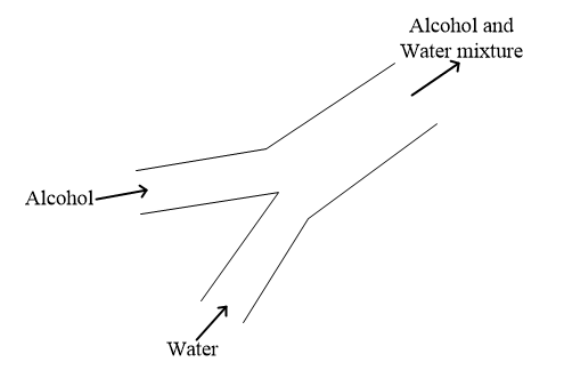
\includegraphics[width=0.75\columnwidth]{figs/B/fig10.png}
\caption{Mixing in Y-channel}
\label{fig:figs/B/fig10.png}
\end{figure}
\hfill{(GATE 2023 XE)}

% Q17
\item The velocity and acceleration of a fluid particle are given as $\vec{V}=(-\hat{i}+2\hat{j})$ m/s
and $\vec{a}=(-2\hat{i}-4\hat{j})$ m/s$^2$, respectively. The magnitude of the component of
acceleration (in m/s$^2$, rounded off to two decimal places) of the fluid particle
along the streamline is \_\_\_\_\_\_.\\
\hfill{(GATE 2023 XE)}

\newpage

% Q18 
\item A hydraulic turbine with rotor diameter of 100 mm produces 200 W of power
while rotating at 300 rpm. Another dynamically-similar turbine rotates at a speed
of 1500 rpm. Consider both turbines to operate with the same fluid (identical density
and viscosity), and neglect any gravitational effect. Then the power (in W,
rounded off to nearest integer) produced by the second turbine is \_\_\_\_\_. \\
\hfill{(GATE 2023 XE)}

% Q19
\item Water (density = 1000 kg/m$^3$) flows steadily with a flow rate of 0.05 m$^3$/s through
a venturimeter having throat diameter of 100 mm. If the pipe diameter is 200 mm
and losses are negligible, the pressure drop (in kPa, rounded off to one decimal
place) between an upstream location in the pipe and the throat (both at the same
elevation) is \_\_\_\_\_\_.\\
\hfill{(GATE 2023 XE)}

% Q20
\item Water flows around a thin flat plate (0.25 m long, 2 m wide) with a free stream
velocity ($U_\infty$) of 1 m/s, as shown in the figure. Consider linear velocity profile
$\left(\dfrac{u}{U_\infty}=\dfrac{y}{\delta}\right)$ for which the laminar boundary layer thickness is expressed as
$\delta=\dfrac{3.5x}{\sqrt{Re_x}}$. For water, density = 1000 kg/m$^3$ and dynamic viscosity = 0.001
kg/m.s. Net drag force (in N, rounded off to two decimal places) acting on the
plate, neglecting the end effects, is \_\_\_\_\_\_.\\

\begin{figure}[htbp]
\centering
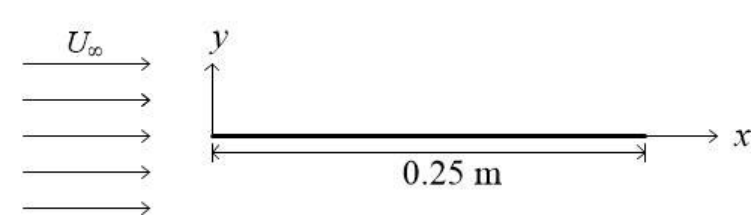
\includegraphics[width=0.8\columnwidth]{figs/B/fig11.png}
\caption{Flow over thin flat plate}
\label{fig:figs/B/fig11.png}
\end{figure}
\hfill{(GATE 2023 XE)}

% Q21
\item Axial velocity profile $u(r)$ for an axisymmetric flow through a circular tube of
radius $R$ is given as, $\dfrac{u(r)}{U}=\left(1-\dfrac{r}{R}\right)^{1/n}$ where $U$ is the centerline velocity. If $V$
refers to the area-averaged velocity (volume flow rate per unit area), then the ratio
$V/U$ for $n=1$ (rounded off to two decimal places) is \_\_\_\_\_.\\
\hfill{(GATE 2023 XE)}

\newpage

% Q22
\item A stationary circular pipe of radius $R=0.5$ m is half filled with water (density =
1000 kg/m$^3$), whereas the upper half is filled with air at atmospheric pressure, as
shown in the figure. Acceleration due to gravity is $g=9.81$ m/s$^2$. The magnitude
of the force per unit length (in kN/m, rounded off to one decimal place) applied by
water on the pipe section AB is \_\_\_\_\_\_.\\

\begin{figure}[htbp]
\centering
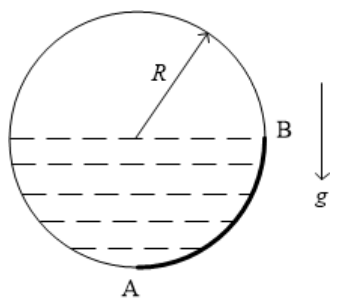
\includegraphics[width=0.5\columnwidth]{figs/B/fig12.png}
\caption{Hydrostatic force on pipe section AB}
\label{fig:figs/B/fig12.png}
\end{figure}
\hfill{(GATE 2023 XE)}

\end{enumerate}

\begin{center}

\item[\textbf{END OF SECTION-B}]

\end{center}

\newpage

%---------------------SECTION-C---------------

\section*{Solid Mechanics}

\begin{enumerate}

\item A plane truss is simply supported at P and R as shown. A downward force $F$ is
applied at hinge Q. The axial force developed in member PS is

\begin{figure}[htbp]
\centering
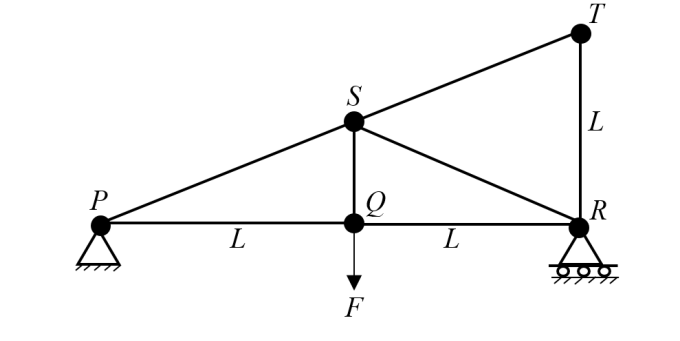
\includegraphics[width=0.75\columnwidth]{figs/C/fig1.png}
\caption{Plane truss with supports at P and R, load at Q}
\label{fig:figs/C/fig1.png}
\end{figure}
\hfill{(GATE 2023 XE)}
\begin{multicols}{2}
\begin{enumerate}
\item $\dfrac{\sqrt{5}}{2}\,F$ Tensile
\item $\dfrac{\sqrt{5}}{2}\,F$ Compressive
\item $\sqrt{5}\,F$ Tensile
\item $\sqrt{5}\,F$ Compressive
\end{enumerate}
\end{multicols}


\item A massless rigid rod OP of length $L$ is hinged frictionlessly at O. A concentrated
mass $m$ is attached to end P of the rod. Initially, the rod OP is horizontal. Then, it
is released from rest. There is gravity as shown. The rod acquires an angular
velocity as it swings. The clockwise angular velocity of the rod, when it first
reaches the vertical position as shown, is

\begin{figure}[htbp]
\centering
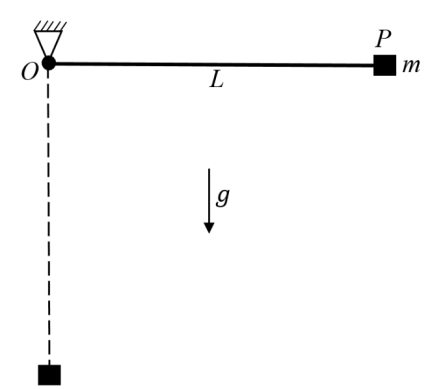
\includegraphics[width=0.3\columnwidth]{figs/C/fig2.png}
\caption{Pendulum-like rigid rod OP with mass m at P}
\label{fig:figs/C/fig2.png}
\end{figure}
\hfill{(GATE 2023 XE)}
\begin{multicols}{4}
\begin{enumerate}
\item $2\sqrt{\dfrac{g}{L}}$
\item $\sqrt{\dfrac{2g}{L}}$
\item $\sqrt{\dfrac{g}{L}}$
\item $\dfrac{1}{2}\sqrt{\dfrac{g}{L}}$
\end{enumerate}
\end{multicols}

\newpage

\item Two equivalent descriptions of the state of stress at a point are shown in the
figure. The normal stresses $\sigma_1$ and $\sigma_2$ as shown on the right must be,
respectively,

\begin{figure}[htbp]
\centering
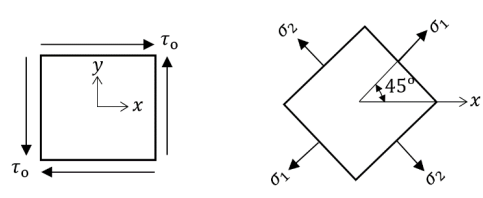
\includegraphics[width=0.4\columnwidth]{figs/C/fig3.png}
\caption{Equivalent stress states at a point}
\label{fig:figs/C/fig3.png}
\end{figure}
\hfill{(GATE 2023 XE)}
\begin{multicols}{2}
\begin{enumerate}
\item $\tau_0$ and $-\tau_0$
\item $-\tau_0$ and $\tau_0$
\item $\dfrac{\tau_0}{\sqrt{2}}$ and $-\dfrac{\tau_0}{\sqrt{2}}$
\item $-\dfrac{\tau_0}{\sqrt{2}}$ and $\dfrac{\tau_0}{\sqrt{2}}$
\end{enumerate}
\end{multicols}

\item The state of strain at a point in a machine component is given as
$\varepsilon_{xx}=2.5\times 10^{-4}$, $\varepsilon_{yy}=2.0\times 10^{-4}$, $\varepsilon_{zz}=-1.5\times 10^{-4}$,
$\varepsilon_{xy}=2.5\times 10^{-4}$, $\varepsilon_{yz}=-0.5\times 10^{-4}$, $\varepsilon_{zx}=-1.0\times 10^{-4}$.
The volumetric strain at this point is\\
\hfill{(GATE 2023 XE)}

\begin{multicols}{2}
\begin{enumerate}
\item $4\times 10^{-4}$
\item $3\times 10^{-4}$
\item $-5\times 10^{-4}$
\item $-3\times 10^{-4}$
\end{enumerate}
\end{multicols}

\item A thin walled, closed cylindrical vessel of inside diameter $d$ and wall thickness $t$
contains a fluid under pressure $p$. The figure below shows a part of the cylindrical
vessel; end caps are not shown. Consider the small element shown with sides
parallel and perpendicular to the axis of the cylinder. The stresses $\sigma_1$ and $\sigma_2$ are
\hfill{(GATE 2023 XE)}

\begin{figure}[htbp]
\centering
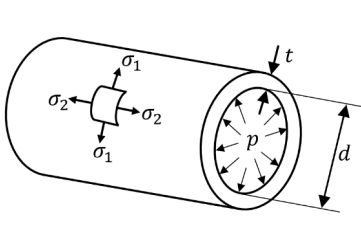
\includegraphics[width=0.4\columnwidth]{figs/C/fig4.png}
\caption{Thin-walled cylinder element and stresses}
\label{fig:figs/C/fig4.png}
\end{figure}

\begin{multicols}{2}
\begin{enumerate}
\item $\sigma_1=\dfrac{pd}{2t};\ \sigma_2=\dfrac{pd}{4t}$
\item $\sigma_1=\dfrac{pd}{t};\ \sigma_2=\dfrac{pd}{2t}$
\item $\sigma_1=\dfrac{pd}{4t};\ \sigma_2=\dfrac{pd}{2t}$
\item $\sigma_1=\dfrac{pd}{2t};\ \sigma_2=0$
\end{enumerate}
\end{multicols}

\newpage

\item A spring mass system is shown in the figure below. Take the acceleration due to
gravity as $g=9.81$ m/s$^2$. The static deflection due to weight and the time period of
oscillations, respectively, are
\hfill{(GATE 2023 XE)}

\begin{figure}[htbp]
\centering
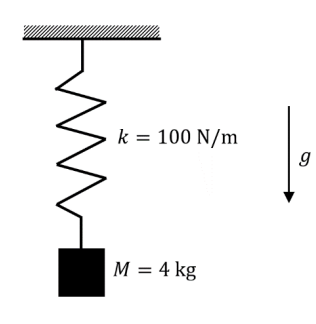
\includegraphics[width=0.4\columnwidth]{figs/C/fig5.png}
\caption{Spring–mass system}
\label{fig:figs/C/fig5.png}
\end{figure}

\begin{multicols}{2}
\begin{enumerate}
\item 0.392 m and 1.26 s
\item 0.392 m and 3.52 s
\item 0.626 m and 1.26 s
\item 0.626 m and 3.52 s
\end{enumerate}
\end{multicols}

\item A rod is subjected to three forces as shown in the figure on the left. An equivalent
force system with forces $F_1$, $F_2$ and moment $M$ is shown in the figure on the
right. The value of $M$ (in N-m) is\_\_\_\_\_\_(rounded off to one decimal place).
\hfill{(GATE 2023 XE)}

\begin{figure}[htbp]
\centering
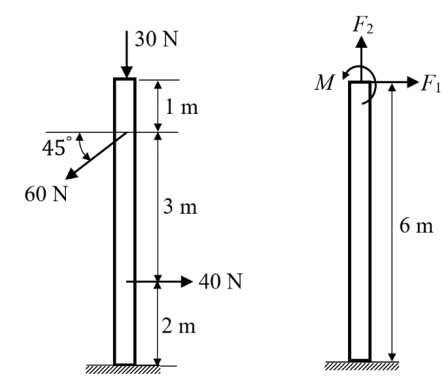
\includegraphics[width=0.4\columnwidth]{figs/C/fig6.png}
\caption{Original and equivalent force systems on a rod}
\label{fig:figs/C/fig6.png}
\end{figure}

\newpage

\item A simply supported beam of length 3 m is loaded as shown in the figure. The
magnitude of the shear force (in kN) at the mid-point of the beam
is \_\_\_\_\_\_(rounded off to one decimal place).


\begin{figure}[htbp]
\centering
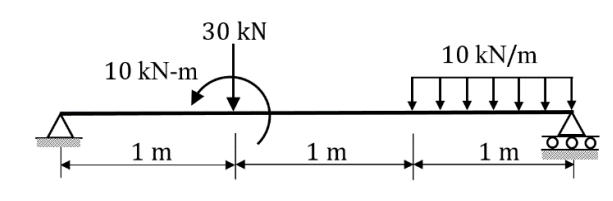
\includegraphics[width=0.6\columnwidth]{figs/C/fig7.png}
\caption{Simply supported beam with loading}
\label{fig:figs/C/fig7.png}
\end{figure}
\hfill{(GATE 2023 XE)}

\item For a plane stress problem, the principal stresses are 100 MPa and 50 MPa. The
magnitude of maximum shear stress (in MPa) in the material is \_\_\_\_\_\_(rounded off to one decimal place).\\
\hfill{(GATE 2023 XE)}

\item A solid uniform rigid disk of mass $m$ and radius $R$ rolls without slipping along a
horizontal surface PQ. The speed of the center of the disk is $v$. The disk then
strikes a hurdle of height $\dfrac{3R}{20}$ at point S. During the impact, there is no rebound or
slip at S and no impulse from the surface PQ. The magnitude of the velocity of the
center of the disk immediately after the impact is\\

\begin{figure}[htbp]
\centering
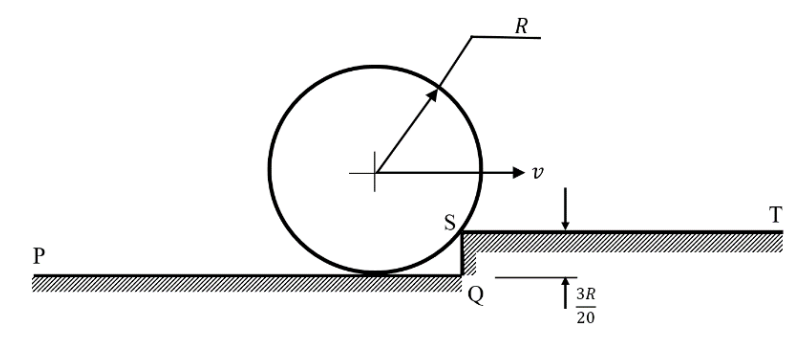
\includegraphics[width=0.7\columnwidth]{figs/C/fig8.png}
\caption{Rolling disk striking a hurdle}
\label{fig:figs/C/fig8.png}
\end{figure}
\hfill{(GATE 2023 XE)}
\begin{multicols}{2}
\begin{enumerate}
\item $0.1v$
\item $0.3v$
\item $0.7v$
\item $0.9v$
\end{enumerate}
\end{multicols}

\newpage

\item A cylinder made of rubber (length $=L$ and diameter $=d$) is inserted in a rigid
container as shown in the figure. The rubber cylinder fits snugly in the rigid
container. There is no wall friction. The modulus of elasticity of the rubber is $E$
and its Poisson’s ratio is $\nu$. The cylinder is subjected to a small uniform pressure $p$
as shown in the figure. The resulting axial strain $(\varepsilon_{zz})$ is\\

\begin{figure}[htbp]
\centering
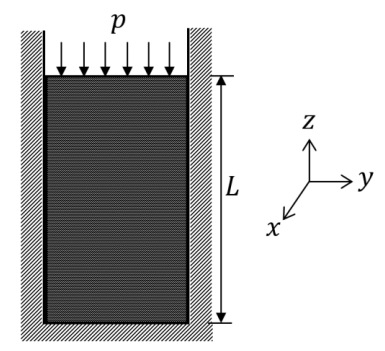
\includegraphics[width=0.4\columnwidth]{figs/C/fig9.png}
\caption{Rubber cylinder confined in rigid container under pressure}
\label{fig:figs/C/fig9.png}
\end{figure}
\hfill{(GATE 2023 XE)}
\begin{multicols}{2}
\begin{enumerate}
\item $-\dfrac{p}{E}$
\item $-\dfrac{p}{E(1-2\nu)}$
\item $-\dfrac{p}{E}\,\dfrac{(1+\nu)(1-2\nu)}{(1-\nu)}$
\item $-\dfrac{p}{E}\,\dfrac{(1-\nu)(1-2\nu)}{(1+\nu)}$
\end{enumerate}
\end{multicols}

\item The state of stress at the critical location in a structure is $\sigma_{xx}=420$ MPa,
$\sigma_{yy}=100$ MPa, $\sigma_{zz}=\sigma_{xy}=\sigma_{yz}=\sigma_{zx}=0$. The yield stress of the material in
uniaxial tension is 400 MPa. Select the correct statement among the following.
\hfill{(GATE 2023 XE)}

\begin{multicols}{2}
\begin{enumerate}
\item The structure is safe by both Tresca (maximum shear stress) theory and von-Mises (distortion energy) theory.
\item The structure is safe by Tresca (maximum shear stress) theory and unsafe by von-Mises (distortion energy) theory.
\item The structure is unsafe by Tresca (maximum shear stress) theory and safe by von-Mises (distortion energy) theory.
\item The structure is unsafe by both Tresca (maximum shear stress) theory and von-Mises (distortion energy) theory.
\end{enumerate}
\end{multicols}

\newpage

\item The figure shows a column of rectangular cross section 100 mm $\times$ 80 mm. It
carries a load of 60 kN at a point 30 mm from the edge $PQ$. The values of stress
component $\sigma_{zz}$ on surfaces $PQQ'P'$ and $SRR'S'$, at points far away from both
ends of the column, are respectively\\

\begin{figure}[htbp]
\centering
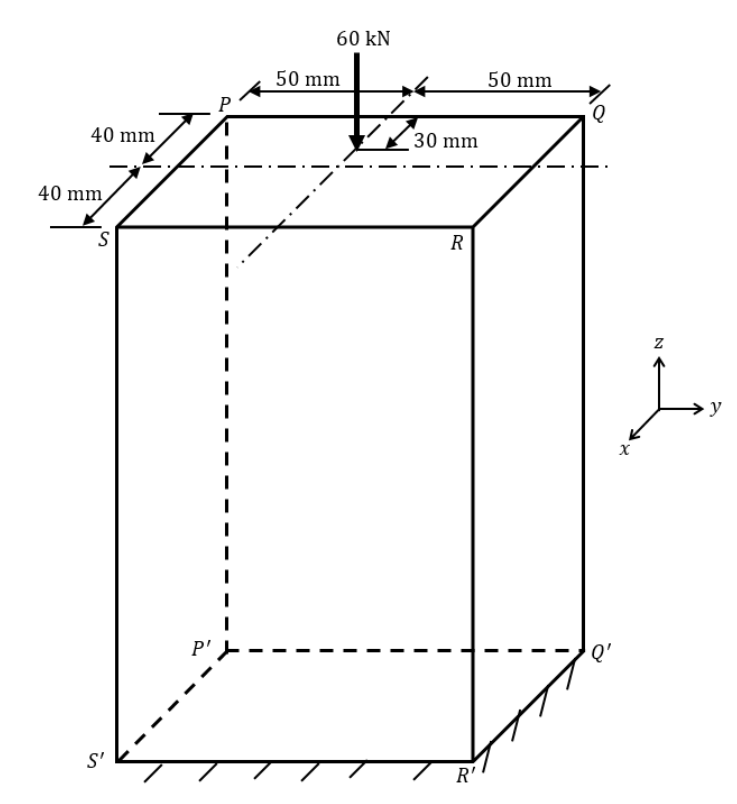
\includegraphics[width=0.4\columnwidth]{figs/C/fig10.png}
\caption{Eccentrically loaded rectangular column}
\label{fig:figs/C/fig10.png}
\end{figure}
\hfill{(GATE 2023 XE)}
\begin{multicols}{2}
\begin{enumerate}
\item 18.75 N/mm$^2$ (Compressive) and 3.75 N/mm$^2$ (Tensile)
\item 18.75 N/mm$^2$ (Compressive) and 3.75 N/mm$^2$ (Compressive)
\item 13.13 N/mm$^2$ (Compressive) and 1.88 N/mm$^2$ (Tensile)
\item 13.13 N/mm$^2$ (Compressive) and 1.88 N/mm$^2$ (Compressive)
\end{enumerate}
\end{multicols}

\item Consider an electric pole with dimensions as shown in the figure. Let the end R be
subjected to a vertical force $F$. The flexural rigidity of both vertical and horizontal
bars is $EI$. Neglect the axial deflection of the vertical bar, and all effects of
self-weight. The vertical deflection at end R is\\

\begin{figure}[htbp]
\centering
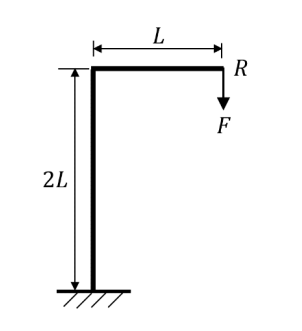
\includegraphics[width=0.2\columnwidth]{figs/C/fig11.png}
\caption{Frame representing an electric pole under load at R}
\label{fig:figs/C/fig11.png}
\end{figure}
\hfill{(GATE 2023 XE)}
\begin{multicols}{2}
\begin{enumerate}
\item $\dfrac{7FL^3}{3EI}$
\item $\dfrac{10FL^3}{3EI}$
\item $\dfrac{5FL^3}{3EI}$
\item $\dfrac{8FL^3}{3EI}$
\end{enumerate}
\end{multicols}


\item A uniform cantilever beam has flexural rigidity $EI$ and length $L$. It is subjected to
a concentrated force $F$ and moment $M=2FL$ at the free end as shown. The
deflection $(\delta)$ at the free end is

\begin{figure}[htbp]
\centering
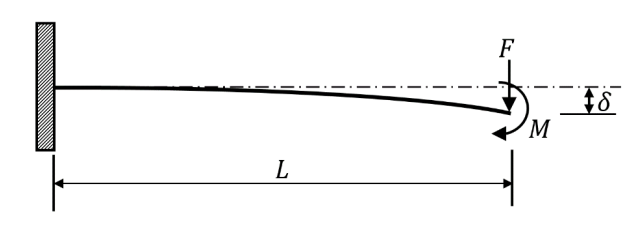
\includegraphics[width=0.5\columnwidth]{figs/C/fig12.png}
\caption{Cantilever with end force $F$ and end moment $2FL$}
\label{fig:figs/C/fig12.png}
\end{figure}
\hfill{(GATE 2023 XE)}
\begin{multicols}{2}
\begin{enumerate}
\item $\dfrac{11FL^3}{12EI}$
\item $\dfrac{8FL^3}{9EI}$
\item $\dfrac{4FL^3}{3EI}$
\item $\dfrac{7FL^3}{6EI}$
\end{enumerate}
\end{multicols}

\item A steel ball of mass $m=10$ kg is suspended from the ceiling of a moving carriage
by two inextensible strings making $60^\circ$ with the horizontal as shown. The carriage
has an acceleration $a$ such that the tension in the string on the right is double the
tension in the string on the left. Take the acceleration due to gravity $(g)$ as 10 m/s$^2$.
The acceleration $a$ (in m/s$^2$) is \_\_\_\_\_\_(rounded off to one decimal place).

\begin{figure}[htbp]
\centering
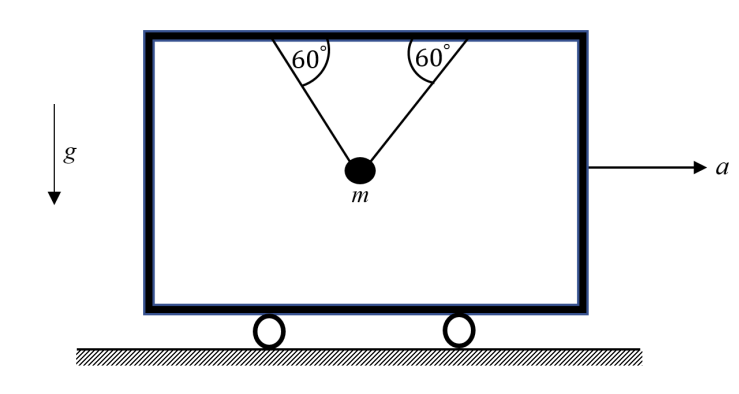
\includegraphics[width=0.5\columnwidth]{figs/C/fig13.png}
\caption{Mass suspended by two strings in an accelerating carriage}
\label{fig:figs/C/fig13.png}
\end{figure}
\hfill{(GATE 2023 XE)}

\newpage

\item A block of mass $m=10$ kg is lying on an inclined plane PQ. The mass is
restrained from sliding down the inclined plane by a force $F$. The coefficient of
friction between the block and the inclined plane is 0.3. Take the acceleration due
to gravity as 10 m/s$^2$. The smallest force $F$ (in N) required to prevent the block
from sliding down is \_\_\_\_\_ (rounded off to one decimal place).\\

\begin{figure}[htbp]
\centering
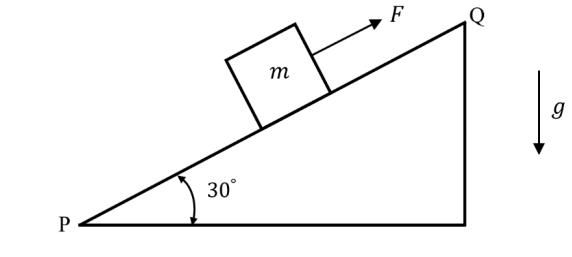
\includegraphics[width=0.5\columnwidth]{figs/C/fig14.png}
\caption{Block on rough inclined plane held by force $F$}
\label{fig:figs/C/fig14.png}
\end{figure}
\hfill{(GATE 2023 XE)}

\item A spherical rigid ball of mass 10 kg is moving with a speed of 2 m/s in the
direction shown. The ball collides with a rigid frictionless wall and rebounds at an
angle $\alpha$ with a speed of $v$, as shown. The coefficient of restitution is 0.9. The
angle $\alpha$ (in degrees) is \_\_\_\_\_\_ (rounded off to one decimal place).\\

\begin{figure}[htbp]
\centering
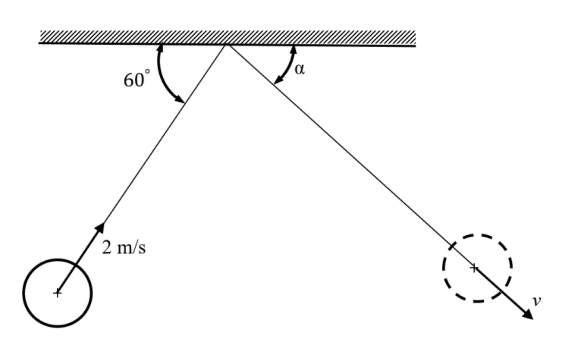
\includegraphics[width=0.4\columnwidth]{figs/C/fig15.png}
\caption{Oblique impact of a ball with a frictionless wall}
\label{fig:figs/C/fig15.png}
\end{figure}
\hfill{(GATE 2023 XE)}

\newpage

\item A thin steel plate is loaded in the x-y plane as shown in the figure. Take the
Poisson’s ratio of steel to be 0.3 and the modulus of elasticity of steel to be 200
GPa. The strain along the $z$-direction is $\varepsilon_{zz}=-3\times 10^{-4}$. The value of
$\sigma_{yy}$ (in MPa) is \_\_\_\_\_\_(rounded off to one decimal place).

\begin{figure}[htbp]
\centering
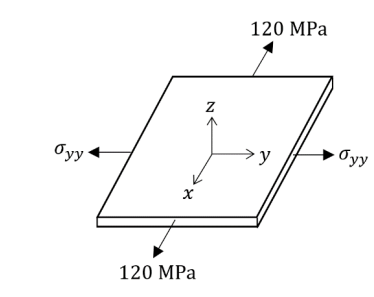
\includegraphics[width=0.4\columnwidth]{figs/C/fig16.png}
\caption{In-plane loading of a thin steel plate}
\label{fig:figs/C/fig16.png}
\end{figure}
\hfill{(GATE 2023 XE)}

\item A composite rod made of steel and copper is fixed immovably at its ends as shown
in the figure. The length of each portion of the rod is 1 m as shown. The
cross-sections of both portions are the same. The moduli of elasticity of steel and
copper are 200 GPa and 100 GPa, respectively. The coefficients of thermal
expansion of steel and copper are $12\times 10^{-6}/^{\circ}C$ and $18\times 10^{-6}/^{\circ}C$, respectively.
The composite rod is initially stress free. Then, the temperature of the composite
rod is increased by $100^{\circ}C$. The magnitude of axial stress (in MPa) developed in
the steel rod is \_\_\_\_\_\_ (rounded off to one decimal place).

\begin{figure}[htbp]
\centering
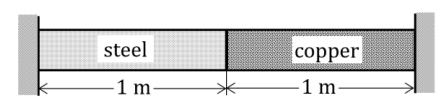
\includegraphics[width=0.4\columnwidth]{figs/C/fig17.png}
\caption{Bi-material composite rod fixed at ends}
\label{fig:figs/C/fig17.png}
\end{figure}
\hfill{(GATE 2023 XE)}\\

\item A slender uniform elastic rod of length 1 m and of solid circular cross-section of
diameter 50 mm is originally straight. It is then loaded by equal and opposite end
moments as indicated in the figure. The resulting lateral displacement of the
mid-point of the rod is 10 mm (displacements are exaggerated in the figure). The
maximum longitudinal strain in the rod is $p\times 10^{-3}$, where $p$ is \_\_\_\_\_\_ (rounded off to one decimal place).

\begin{figure}[htbp]
\centering
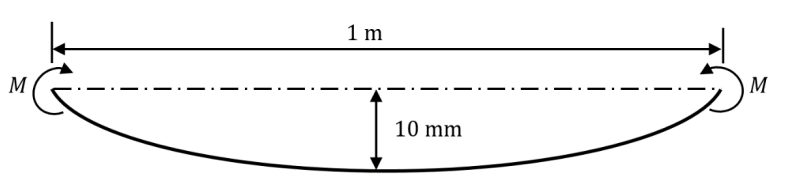
\includegraphics[width=0.6\columnwidth]{figs/C/fig18.png}
\caption{Slender elastic rod under equal and opposite end moments}
\label{fig:figs/C/fig18.png}
\end{figure}
\hfill{(GATE 2023 XE)}\\

\item Consider a solid cylindrical shaft and a hollow cylindrical shaft. Both shafts are
axisymmetric and elastic, and have the same cross-sectional area. The hollow
shaft has an outside diameter of 150 mm and an inside diameter of 120 mm. When
both the shafts are twisted by the same twisting moment, the ratio of maximum
shear stress developed in the hollow shaft $(\tau_h)$ to maximum shear stress
developed in the solid shaft $(\tau_s)$ will be \_\_\_\_\_\_ (rounded off to three decimal places).\\
\hfill{(GATE 2023 XE)}

\end{enumerate}



\begin{center}

\item[\textbf{END OF SECTION-C}]

\end{center}

\newpage

%---------------------SECTION-D---------------

\section*{Thermodynamics}
\bigskip

\begin{enumerate}

\item A: The number of properties required to fix the state of a system is given by ‘state postulate’. \\
R: The state of a simple compressible system is completely specified by two independent, intensive properties. \\
About the statements A and R applied to a single-phase system,
\hfill{(GATE 2023 XE)}

\begin{multicols}{2}
\begin{enumerate}
\item A is correct and R is incorrect.
\item A is incorrect and R is correct.
\item Both A and R are incorrect.
\item Both A and R are correct.
\end{enumerate}
\end{multicols}

\item Which of the following is an extensive property of a system?
\hfill{(GATE 2023 XE)}

\begin{multicols}{2}
\begin{enumerate}
\item Density
\item Pressure
\item Temperature
\item Total mass
\end{enumerate}
\end{multicols}

\item A tank of volume $V$ contains homogeneous mixture of two ideal gases, A and B at a temperature $T$ and a pressure $P$. The mixture contains $n_A$ moles of gas A and $n_B$ moles of gas B. If $P_A$ and $P_B$ are the partial pressures of gas A and gas B, respectively, then
\hfill{(GATE 2023 XE)}

\begin{multicols}{2}
\begin{enumerate}
\item $P_A=\dfrac{n_A}{n_A+n_B}P,\quad P_B=\dfrac{n_B}{n_A+n_B}P$
\item $P_A=\dfrac{n_B}{n_A}P,\quad P_B=\dfrac{n_A}{n_B}P$
\item $P_A=\dfrac{n_A}{n_B}P,\quad P_B=\dfrac{n_B}{n_A}P$
\item $P_A=\dfrac{n_B}{n_A+n_B}P,\quad P_B=\dfrac{n_A}{n_A+n_B}P$
\end{enumerate}
\end{multicols}

\item If an ideal air-standard Otto cycle and an ideal air-standard Diesel cycle operate on the same compression ratio, then the relation between the thermal efficiencies $(\eta_{th})$ of the cycles is
\hfill{(GATE 2023 XE)}

\begin{multicols}{2}
\begin{enumerate}
\item $\eta_{th,\text{Otto}}=\eta_{th,\text{Diesel}} \ \text{and}\ \eta_{th,\text{Otto}}<1$
\item $\eta_{th,\text{Otto}}>\eta_{th,\text{Diesel}}$
\item $\eta_{th,\text{Otto}}<\eta_{th,\text{Diesel}}$
\item $\eta_{th,\text{Otto}}=\eta_{th,\text{Diesel}}=1$
\end{enumerate}
\end{multicols}

\item The following statements are given: \\
(i) The third law of thermodynamics deals with the entropy of a substance at the absolute zero temperature. \\
(ii) Entropy of any non-crystalline structure is zero at absolute zero temperature. \\
(iii) At the absolute zero temperature, the crystal structure has maximum degree of order. \\
(iv) The thermal energy of the substance at absolute zero temperature is maximum. \\
The correct option describing these statements is
\hfill{(GATE 2023 XE)}

\begin{multicols}{2}
\begin{enumerate}
\item Only (i) is correct
\item Only (ii) is correct
\item Both (i) and (iii) are correct
\item Both (i) and (iv) are correct
\end{enumerate}
\end{multicols}

\item Adiabatic bulk modulus of a substance is defined as
\hfill{(GATE 2023 XE)}

\begin{multicols}{2}
\begin{enumerate}
\item $-\dfrac{1}{v}\left(\dfrac{\partial v}{\partial P}\right)_T$
\item $-v\left(\dfrac{\partial P}{\partial v}\right)_T$
\item $-\dfrac{1}{v}\left(\dfrac{\partial v}{\partial P}\right)_s$
\item $-v\left(\dfrac{\partial P}{\partial v}\right)_s$
\end{enumerate}
\end{multicols}

\newpage

\item An insulated rigid closed tank of $2\,\mathrm{m^3}$ internal volume contains saturated liquid-vapor mixture of water at $200^{\circ}\mathrm{C}$. The quality of the mixture is $0.75$. The mass of the mixture in the tank is \_\_\_\_\_\_\_\_\_\_\_\_ kg (rounded off to one decimal place). \\
\hfill{(GATE 2023 XE)}

\item A rigid closed tank contains $2\,\mathrm{kg}$ of an ideal gas at $500\,\mathrm{kPa}$ and $350\,\mathrm{K}$. A valve is opened, and half of the mass of the gas is allowed to escape. Then the valve is closed. If the final pressure in the tank is $300\,\mathrm{kPa}$, the final temperature in the tank is \_\_\_\_\_\_\_\_\_\_\_\_ K (in integer).
\hfill{(GATE 2023 XE)}

\item Air at $400\,\mathrm{K}$ and $200\,\mathrm{kPa}$ is heated at constant pressure to $600\,\mathrm{K}$. Assuming that the internal energy is a function of temperature only, the magnitude of change in internal energy during this process is \_\_\_\_\_\_\_\_\_\_\_\_ kJ/kmol (rounded off to one decimal place). \\
\hfill{(GATE 2023 XE)}

\item A rigid closed tank having a volume of $2\,\mathrm{m^3}$ contains $0.1\,\mathrm{m^3}$ of saturated liquid water and $1.9\,\mathrm{m^3}$ of saturated water vapor at $100\,\mathrm{kPa}$. Heat is transferred to the tank until the final tank pressure reaches $2\,\mathrm{MPa}$. \\
Following data for water is given: \\
At $100\,\mathrm{kPa}$: $v_f=0.001043\,\mathrm{m^3/kg}$, $v_g=1.694\,\mathrm{m^3/kg}$, $u_f=417.33\,\mathrm{kJ/kg}$, $u_g=2506.06\,\mathrm{kJ/kg}$ \\
At $2\,\mathrm{MPa}$: $v_f=0.001177\,\mathrm{m^3/kg}$, $v_g=0.09963\,\mathrm{m^3/kg}$, $u_f=906.42\,\mathrm{kJ/kg}$, $u_g=2600.26\,\mathrm{kJ/kg}$ \\
The magnitude of heat transfer in this process is\\
\hfill{(GATE 2023 XE)}

\begin{multicols}{2}
\begin{enumerate}
\item 34670 kJ
\item 55842 kJ
\item 67906 kJ
\item 77470 kJ
\end{enumerate}
\end{multicols}

\item An ideal Diesel cycle has a compression ratio of 20 and cut-off ratio of 1.5. At the beginning of the compression stroke, air is at $100\,\mathrm{kPa}$, $300\,\mathrm{K}$. Use the cold-air-standard assumptions with property value $c_p=1.005\,\mathrm{kJ/kg\text{-}K}$. Assume $c_p/c_v=1.4$. For this cycle, the net work output per unit mass is\\
\hfill{(GATE 2023 XE)}

\begin{multicols}{2}
\begin{enumerate}
\item 335 kJ/kg
\item 395 kJ/kg
\item 500 kJ/kg
\item 165 kJ/kg
\end{enumerate}
\end{multicols}



\item A $5\,\mathrm{kg}$ metal block ($c_p=0.5\,\mathrm{kJ/kg\text{-}K}$) at $373\,\mathrm{K}$ is submerged into $10\,\mathrm{kg}$ of water ($c_p=4.2\,\mathrm{kJ/kg\text{-}K}$) at $293\,\mathrm{K}$ in an insulated rigid container without spilling. Assuming thermal equilibrium is reached, the approximate entropy change of the universe is\\
\hfill{(GATE 2023 XE)}

\begin{multicols}{2}
\begin{enumerate}
\item $-0.565$ kJ/K
\item $0.073$ kJ/K
\item $0.642$ kJ/K
\item $0.963$ kJ/K
\end{enumerate}
\end{multicols}

\newpage


\item Match the following: \\

\begin{tabular}[12pt]{ |c| c| c| c| }
\hline
$\beta$ & Airplane A & Airplane B & Airplane C \\
\hline
$\beta = -5\,\mathrm{deg}$ & $-0.030$ & $-0.025$ & $0.040$\\
\hline
$\beta = 0\,\mathrm{deg}$ & $0$ & $0$ & $0$ \\
\hline
$\beta = 5\,\mathrm{deg}$ & $0.030$ & $0.025$ & $-0.040$\\
\hline
\end{tabular}


\hfill{(GATE 2023 XE)}

\begin{multicols}{2}
\begin{enumerate}
\item A1$\rightarrow$B2, A2$\rightarrow$B4, A3$\rightarrow$B1, A4$\rightarrow$B3
\item A1$\rightarrow$B4, A2$\rightarrow$B2, A3$\rightarrow$B1, A4$\rightarrow$B3
\item A1$\rightarrow$B2, A2$\rightarrow$B4, A3$\rightarrow$B3, A4$\rightarrow$B1
\item A1$\rightarrow$B4, A2$\rightarrow$B2, A3$\rightarrow$B3, A4$\rightarrow$B1
\end{enumerate}
\end{multicols}


\item A piston-cylinder device initially contains $1\,\mathrm{m^3}$ of air at $200\,\mathrm{kPa}$ and $25^{\circ}\mathrm{C}$. Air expands at constant pressure while a heater of $250\,\mathrm{W}$ is switched on for 10 minutes. There is a heat loss of $4\,\mathrm{kJ}$ during this process. Assuming air as an ideal gas, the final temperature of air is \_\_\_\_\_\_\_ $^{\circ}\mathrm{C}$ (rounded off to one decimal place). \\
Use the following data for air: $R=0.287\,\mathrm{kJ/kg\text{-}K}$, $c_p=1.005\,\mathrm{kJ/kg\text{-}K}$
\hfill{(GATE 2023 XE)}\\

\item Steam at $2\,\mathrm{MPa}$ and $300^{\circ}\mathrm{C}$ steadily enters a nozzle of inlet diameter of $20\,\mathrm{cm}$. Steam leaves the nozzle with a velocity of $300\,\mathrm{m/s}$. The mass flow rate of steam through the nozzle is $10\,\mathrm{kg/s}$. Assume no work interaction and no change in potential energy. If the heat loss from the nozzle per kg of steam is $3\,\mathrm{kJ}$, the exit enthalpy per kg of steam is \_\_\_\_\_\_\_\_\_ kJ (rounded off to nearest integer). \\
Use the following data for steam: At $2\,\mathrm{MPa}$ and $300^{\circ}\mathrm{C}$: $v=0.12551\,\mathrm{m^3/kg}$, $h=3024.2\,\mathrm{kJ/kg}$
\hfill{(GATE 2023 XE)}\\

\item A rigid tank of $2\,\mathrm{m^3}$ internal volume contains $5\,\mathrm{kg}$ of water as a saturated liquid-vapor mixture at $400\,\mathrm{kPa}$. Half of the mass of the saturated liquid in the tank is drained-off while maintaining constant pressure of $400\,\mathrm{kPa}$ in the tank. The final quality of the mixture remaining in the tank is \_\_\_\_\_\_\_\_\_\_\_ (rounded off to two decimal places). \\
\hfill{(GATE 2023 XE)}\\

\item Consider a spark ignition engine which operates on an ideal air-standard Otto cycle. It uses a fuel which produces $44\,\mathrm{MJ/kg}$ of heat in the engine. If the engine requires $40\,\mathrm{mg}$ of fuel to produce $1\,\mathrm{kJ}$ of work output, then the compression ratio of the Otto cycle is \_\_\_\_\_\_\_\_\_\_ (rounded off to two decimal places). \\
For the entire cycle, use $c_p/c_v=1.4$
\hfill{(GATE 2023 XE)}\\

\item A refrigerator operates on an ideal vapor compression cycle between the pressure limits of $140\,\mathrm{kPa}$ and $800\,\mathrm{kPa}$. The working fluid is the refrigerant R-134a. The refrigerant enters the compressor as saturated vapor at $140\,\mathrm{kPa}$ and exits at $800\,\mathrm{kPa}$ and $60^{\circ}\mathrm{C}$. It leaves the condenser as a saturated liquid at $800\,\mathrm{kPa}$. The coefficient of performance (COP) of the refrigerator is \_\_\_\_\_\_\_\_\_ (rounded off to two decimal places). \\
\hfill{(GATE 2023 XE)}

\item A steam power plant operates on a simple ideal Rankine cycle. The condenser pressure is $10\,\mathrm{kPa}$ and the boiler pressure is $5\,\mathrm{MPa}$. The steam enters the turbine at $600^{\circ}\mathrm{C}$. Mass flow rate of the steam is $50\,\mathrm{kg/s}$. Neglecting the pump work, the net power output of the plant is \_\_\_\_\_ MW (rounded off to one decimal place). \\
\hfill{(GATE 2023 XE)}

\item In an air-conditioning system, air enters at $20^{\circ}\mathrm{C}$ and 30\% relative humidity at a steady rate of $30\,\mathrm{m^3/min}$ in a humidifier and it is conditioned to $25^{\circ}\mathrm{C}$ and 60\% relative humidity. Assuming entire process takes place at pressure of $100\,\mathrm{kPa}$, the mass flow rate of the steam added to air in the humidifier is \_\_\_\_\_\_\_\_ kg/min (rounded off to three decimal places). \\
\hfill{(GATE 2023 XE)}

\item An office uses a heat pump to receive $500\,\mathrm{kJ/day}$ heat in winter to maintain its temperature at $300\,\mathrm{K}$. The ambient temperature is $280\,\mathrm{K}$. If the COP of the heat pump is 60\% of its theoretical maximum value, the ratio of actual work input to the minimum theoretical work input to the heat pump is \_\_\_\_\_\_\_\_\_ (rounded off to one decimal place).
\hfill{(GATE 2023 XE)}

\item In a liquid-vapour phase change process, $\left(\dfrac{dP}{dT}\right)_{sat}$ at $100^{\circ}\mathrm{C}$ for saturated water is $3750\,\mathrm{Pa/K}$. If the resulting change in specific volume $(v_g-v_f)$ is $1.672\,\mathrm{m^3/kg}$, the enthalpy of vaporization $(h_{fg})$ will be \_\_\_\_\_\_\_\_\_\_\_\_ kJ/kg (in integer).
\hfill{(GATE 2023 XE)}

\end{enumerate}

\begin{center}

\item[\textbf{END OF SECTION-D}]

\end{center}

\newpage

%---------------------SECTION-E---------------

\section*{Polymer Science and Engineering}

\begin{enumerate}

\item Which one of the monomers given is used in the synthesis of cellulose?
\hfill{(GATE 2023 XE)}

\begin{multicols}{2}
\begin{enumerate}
\item Fructose
\item Lactic acid
\item Galactose
\item Glucose
\end{enumerate}
\end{multicols}

\item A copper wire upon loading instantaneously increases in length to l, and then continues to elongate gradually. Upon unloading, the wire retracts to length l. According to the Maxwell model, which one of the options given correctly relates the total strain E, the applied stress S, the modulus G, the material’s resistance to flow $\eta$, and the elapsed time t between loading and unloading?
\hfill{(GATE 2023 XE)}

\begin{multicols}{2}
\begin{enumerate}
\item E = (S/G) – (S/$\eta$)t
\item E = (S/G) × (S/$\eta$)t
\item E = (S/G) + (S/$\eta$)t
\item E = (S/G) / (S/$\eta$)t
\end{enumerate}
\end{multicols}

\item Consider the structure of a cross-linked polymer shown in the figure. From the options given, identify the monomers that are used in the synthesis of the polymer.
\hfill{(GATE 2023 XE)}

\begin{figure}[htbp]
\centering
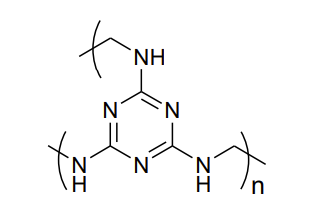
\includegraphics[width=0.3\columnwidth]{figs/E/fig1.png}
\caption{Structure of a crosslinked polymer used to identify constituent monomers}
\label{fig:figs/E/fig1.png}
\end{figure}

\begin{multicols}{2}
\begin{enumerate}
\item Melamine and Benzaldehyde
\item Melamine and Acetone
\item Melamine and Formaldehyde
\item Melamine and Ethanol
\end{enumerate}
\end{multicols}

\item Among the options given, choose the most suitable compatibilizer for blending Polyvinylidene fluoride (PVDF) and Acrylonitrile butadiene styrene (ABS).
\hfill{(GATE 2023 XE)}

\begin{multicols}{2}
\begin{enumerate}
\item Styrene-acrylonitrile (SAN)
\item Polybutadiene (PB)
\item Polymethyl methacrylate (PMMA)
\item Nylon 6
\end{enumerate}
\end{multicols}

\item A high molecular weight polymer passes through different zones from the hopper to the die in an extruder. Among the options given, identify the correct match between the zones and their key functions.
\hfill{(GATE 2023 XE)}

\begin{table}[h!]
\small
\setlength{\tabcolsep}{4pt}
\renewcommand{\arraystretch}{0.9}
\centering
\begin{tabular}{|c|c|c|p{1.8cm}|p{2.5cm}|c|}
\hline
Q. No & Type & Section & Key & Marks \\
\hline
1  & MCQ & GA & C         & 1 \\
\hline
2  & MCQ & GA & A         & 1 \\
\hline
3  & MCQ & GA & A         & 1 \\
\hline
4  & MCQ & GA & A         & 1 \\
\hline
5  & MCQ & GA & D         & 1 \\
\hline
6  & MCQ & GA & D         & \textbf{2} \\
\hline
7  & MCQ & GA & B         & 2 \\
\hline
8  & MCQ & GA & C         & 2 \\
\hline
9  & MCQ & GA & B         & 2 \\
\hline
10 & MCQ & GA & C         & 2 \\
\hline
11 & MCQ & EY & D         & 1 \\
\hline
12 & MCQ & EY & D         & 1 \\
\hline
13 & MCQ & EY & A; D      & 1 \\
\hline
14 & MCQ & EY & B         & 1 \\
\hline
15 & NAT & EY & 7.99 : 8.10 & 1 \\
\hline
16 & MCQ & EY & B         & 1 \\
\hline
17 & MCQ & EY & C         & 1 \\
\hline
18 & MCQ & EY & D         & 1 \\
\hline
19 & NAT & EY & 9.9 : 10.1  & 1 \\
\hline
20 & MCQ & EY & C         & 1 \\
\hline
21 & MCQ & EY & B         & 1 \\
\hline
22 & MCQ & EY & A         & 1 \\
\hline
23 & MCQ & EY & D         & 1 \\
\hline
24 & MCQ & EY & B         & 1 \\
\hline
25 & MCQ & EY & A         & 1 \\
\hline
26 & MCQ & EY & C         & 2 \\
\hline
27 & MCQ & EY & D         & 2 \\
\hline
28 & MCQ & EY & C         & 2 \\
\hline
29 & MCQ & EY & D         & 2 \\
\hline
30 & MCQ & EY & B         & 2 \\
\hline
31 & MCQ & EY & A         & 2 \\
\hline
32 & MCQ & EY & C         & 2 \\
\hline
33 & MCQ & EY & A         & 2 \\
\hline
34 & MCQ & EY & B         & 2 \\
\hline
35 & MCQ & EY & A         & 2 \\
\hline
36 & MCQ & EY & A         & 2 \\
\hline
37 & MCQ & EY & C         & 2 \\
\hline
38 & MCQ & EY & A         & 2 \\
\hline
39 & NAT & EY & 0.17 : 0.19 & 2 \\
\hline
40 & MCQ & EY & A         & 2 \\
\hline
41 & MCQ & EY & B         & 2 \\
\hline
42 & MCQ & EY & B         & 2 \\
\hline
43 & MCQ & EY & A         & 2 \\
\hline
44 & MCQ & EY & D         & 2 \\
\hline
45 & MCQ & EY & B         & 2 \\
\hline
46 & MCQ & EY & A         & 2 \\
\hline
47 & NAT & EY & 0.175 : 0.20 & 2 \\
\hline
48 & MCQ & EY & A         & 2 \\
\hline
49 & NAT & EY & 0.49 : 0.51  & 2 \\
\hline
50 & MCQ & EY & B         & 2 \\
\hline
51 & MCQ & EY & A         & 2 \\
\hline
52 & MCQ & EY & C         & 2 \\
\hline
53 & NAT & EY & 1660 : 1700 & 2 \\
\hline
54 & NAT & EY & 0.45 : 0.55 & 2 \\
\hline
55 & MCQ & EY & A         & 2 \\
\hline
\end{tabular}
\caption{GATE 2016 EY Answer Key Summary}
\end{table}

\begin{multicols}{2}
\begin{enumerate}
\item P-4; Q-3; R-2; S-1
\item P-3; Q-4; R-1; S-2
\item P-4; Q-1; R-2; S-3
\item P-3; Q-1; R-2; S-4
\end{enumerate}
\end{multicols}

\item Polymer wetting is improved by the addition of fillers with functional groups. In a typical case-study, natural-clay was modified with hydroxyl groups and compounded with Nylon 6 along with an antioxidant. The resulting composite exhibited poor mechanical properties. Which one among the options given explains this observation?
\hfill{(GATE 2023 XE)}

\begin{multicols}{2}
\begin{enumerate}
\item The surface functional groups of the filler reacted with Nylon 6
\item The antioxidant degraded during the processing
\item The surface functional groups of the filler formed hydrogen bonds with the antioxidant
\item The antioxidant reacted with Nylon 6
\end{enumerate}
\end{multicols}

\item Among the options given, identify the correct match between the polymers and their glass transition temperatures (Tg).
\hfill{(GATE 2023 XE)}

\begin{center}
\begin{tabular}{|p{1cm}|p{3cm}|p{1cm}|p{7cm}|}
\hline

\multicolumn{2}{|c|}{Process} & \multicolumn{2}{c|}{Application} \\
\hline
P & Extrusion & 1 & Producing complex parts with close tolerance \\
\hline
Q & Injection molding & 2 & Producing thermosetting plastic components \\
\hline
R & Blow molding & 3 & Producing long uniform sections \\
\hline
S & Compression molding & 4 & Producing hollow shapes \\
\hline
\end{tabular}
\end{center}

\begin{multicols}{2}
\begin{enumerate}
\item P-2; Q-4; R-3; S-1
\item P-3; Q-1; R-4; S-2
\item P-3; Q-4; R-1; S-2
\item P-4, Q-2; R-1; S-3
\end{enumerate}
\end{multicols}

\item What is the correct order of decreasing crystallinity of the given polymers?
\hfill{(GATE 2023 XE)}

P\; atactic-Polypropylene \quad Q\; syndiotactic-Polystyrene \\
R\; Nylon 6 \quad S\; Polyethylene terephthalate

\begin{multicols}{2}
\begin{enumerate}
\item P $>$ R $>$ S $>$ Q
\item S $>$ Q $>$ P $>$ R
\item Q $>$ S $>$ R $>$ P
\item S $>$ R $>$ Q $>$ P
\end{enumerate}
\end{multicols}

\newpage

\item Choose the correct option that best correlates the graphs with the polymerization methods.
\hfill{(GATE 2023 XE)}

\begin{figure}[htbp]
\centering
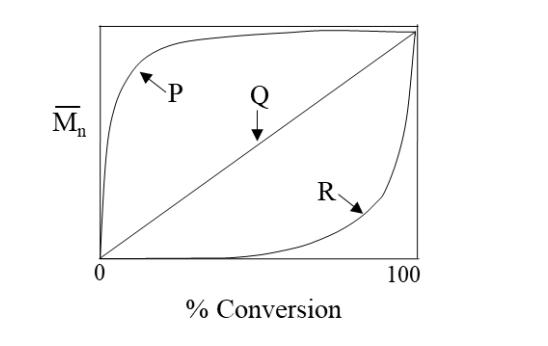
\includegraphics[width=0.4\columnwidth]{figs/E/fig2.png}
\caption{Graphs to be matched with polymerization methods}
\label{fig:figs/E/fig2.png}
\end{figure}

\begin{multicols}{2}
\begin{enumerate}
\item P – living polymerization; Q – chain growth; R – step growth
\item P – chain growth; Q – living polymerization; R – step growth
\item P – step growth; Q – living polymerization; R – chain growth
\item P – living polymerization; Q – step growth; R – chain growth
\end{enumerate}
\end{multicols}

\item From the options given, identify the correct match(es) between the polymer products with the most appropriate processing technique.
\hfill{(GATE 2023 XE)}

\begin{tabular}[12pt]{ |c| c| c| c| c| c| }
    \hline
   Q.No. & Session & Que.Type & Sec. Name & Key & Marks \\
    \hline
    46 & 4 & NAT & AE & 149.0 to 151.0 & 2\\
    \hline
    47 & 4 & NAT & AE & 1712.0 to 1719.0 & 2\\
    \hline
    48 & 4 & NAT & AE & 91 to 93 & 2\\
    \hline
    49 & 4 & NAT & AE & 87 to 89 & 2\\
    \hline
    50 & 4 & NAT & AE & 27.0 to 27.2 & 2\\
    \hline
    51 & 4 & NAT & AE & 1.43 to 1.45 & 2\\
    \hline
    52 & 4 & NAT & AE & 0.61 to 0.63 & 2\\
    \hline
    53 & 4 & NAT & AE & 3.74 to 3.76 & 2\\
    \hline
    54 & 4 & NAT & AE & 62.95 to 63.08 & 2\\
    \hline
    55 & 4 & NAT & AE & 57.10 to 60.00 & 2\\
    \hline
\end{tabular}


\begin{multicols}{2}
\begin{enumerate}
\item P-3; Q-4; R-1; S-2
\item P-3; Q-2; R-1; S-4
\item P-1; Q-2; R-3; S-4
\item P-3; Q-4; R-1; S-1
\end{enumerate}
\end{multicols}

\item Among the options given, which agents are used to vulcanize or cure rubbers?
\hfill{(GATE 2023 XE)}

\begin{multicols}{2}
\begin{enumerate}
\item Dicumyl peroxide
\item Zinc stearate
\item Carbon black
\item Dinitrobenzene
\end{enumerate}
\end{multicols}

\item Lipase is a natural enzyme, which cleaves carboxylic ester bonds. Among the options given, identify the polymer(s) degraded by lipase.
\hfill{(GATE 2023 XE)}

\begin{multicols}{2}
\begin{enumerate}
\item Polypropylene (PP)
\item Polycaprolactone (PCL)
\item Polyvinylidene fluoride (PVDF)
\item Polyethylene terephthalate (PET)
\end{enumerate}
\end{multicols}

\newpage

\item Among the options given, identify the correct pair(s) of catalyst and co-catalyst that form a Ziegler-Natta catalyst.\\
\hfill{(GATE 2023 XE)}

\begin{multicols}{2}
\begin{enumerate}
\item TiCl3 and Al(CH3CH2)2Cl
\item ZnCl2 and Al(CH3)3
\item TiO2 and Al(CH3)3
\item VCl4 and Al(CH3CH2)2Cl
\end{enumerate}
\end{multicols}

\item Mechanical stress is applied on a polymer. Identify the correct match(es) between the statements (1, 2, 3, 4, 5) that describe the deformations and
the regimes (P, Q, R).
\hfill{(GATE 2023 XE)}

\begin{table}[H]
\centering
\begin{tabular}{|c|c|c|c|}
\hline
\textbf{Activity} & \textbf{Optimistic time (days)} & \textbf{Most likely time (days)} & \textbf{Pessimistic time (days)} \\
\hline
1-2 & 1 & 2 & 3 \\
1-3 & 5 & 6 & 7 \\
1-4 & 3 & 5 & 7 \\
2-5 & 5 & 7 & 9 \\
3-5 & 2 & 4 & 6 \\
5-6 & 4 & 5 & 6 \\
4-7 & 4 & 6 & 8 \\
6-7 & 2 & 3 & 4 \\
\hline
\end{tabular}
\caption{Activity Time Estimates}
\end{table}


\begin{multicols}{2}
\begin{enumerate}
\item P-2; Q-5; R-1
\item P-1; Q-5; R-1
\item P-2; Q-3; R-4
\item P-4; Q-3; R-1
\end{enumerate}
\end{multicols}

\item Stress versus elongation profiles for different polymeric materials are shown in the figure. Choose the combination that best describes these profiles.
\hfill{(GATE 2023 XE)}

\begin{figure}[htbp]
\centering
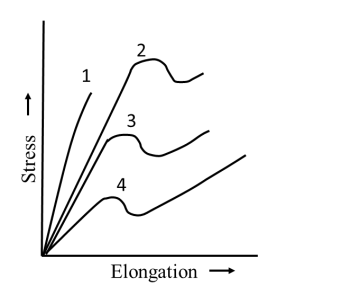
\includegraphics[width=0.4\columnwidth]{figs/E/fig3.png}
\caption{Stress–elongation profiles for different polymeric materials}
\label{fig:figs/E/fig3.png}
\end{figure}

\begin{multicols}{2}
\begin{enumerate}
\item 1-Nylon fibers; 2-Polyethylene; 3-Vulcanized rubber; 4-Polystyrene
\item 1-Polyethylene; 2-Vulcanized rubber; 3-Polystyrene; 4-Nylon fibers
\item 1-Polystyrene; 2-Nylon fibers; 3-Polyethylene; 4-Vulcanized rubber
\item 1-Vulcanized rubber; 2-Polyethylene; 3-Nylon fibers; 4-Polystyrene
\end{enumerate}
\end{multicols}

\item Among the options given, which method(s) is/are used for the synthesis of atactic polystyrene?
\hfill{(GATE 2023 XE)}

\begin{multicols}{2}
\begin{enumerate}
\item Free radical polymerization
\item Ring opening polymerization
\item Polycondensation
\item Ionic polymerization
\end{enumerate}
\end{multicols}

\item A nylon sample of 0.03 m2 cross-sectional area is subjected to a creep load of 10 kN. The load is removed after a duration of 60 s. Young’s modulus and the viscosity for nylon are 1 GPa and 300 Giga Poise. The compliance of the specimen is \_\_\_\_\_\_\_\_ ×10-9 m2/N. (Answer in integer)\\
\hfill{(GATE 2023 XE)}\\

\item Polyvinylidine fluoride (PVDF) was quenched from the melt in one case and in the other case, it was slowly cooled from the melt at 10 °C/min. The percentage crystallinity of the slowly cooled PVDF is 60\%. The heat of fusion for the quenched PVDF is 0.5$\Delta$Hm ($\Delta$Hm is the heat of fusion for the slowly cooled PVDF), and the heat of fusion for 100\% crystalline PVDF is 100 J/g. The percentage crystallinity of the quenched PVDF is \_\_\_\_\_ \%. (Answer in integer)\\
\hfill{(GATE 2023 XE)}\\

\item A polymeric material of density 0.9 g/cc and melt volume of 10 cc in an extruder has a residence time of 100 s. The output of the extruder is \_\_\_\_\_ kg/h. (Rounded off to two decimal places)\\
\hfill{(GATE 2023 XE)}\\

\item A polymer weighing 0.2 g is dissolved in 100 ml of benzene and has a relative viscosity of 1.5. The polymer obeys Mark-Houwink equation with constants a = 0.5 and K = 0.001. The molecular weight of the polymer is \_\_\_\_\_ ×10$^{10}$ g/mol. (Rounded off to two decimal places)\\
\hfill{(GATE 2023 XE)}\\

\item A continuous and aligned glass-fiber reinforced composite consists of 40 vol\% of glass-fiber having a modulus of elasticity of 69 GPa and 60 vol\% of a polyester resin, which when hardened, displays a modulus of 3.4 GPa. The modulus of elasticity of this composite in the longitudinal direction is \_\_\_\_\_\_\_\_\_ GPa.
(Rounded off to two decimal places)\\
\hfill{(GATE 2023 XE)}\\
\begin{center}
\begin{tabular}{|c|c|c|}
\hline
\textbf{Activity} & \textbf{Activity time (in days)} & \textbf{Immediate predecessor(s)} \\
\hline
A & 2 & - \\
B & 3 & - \\
C & 2 & A \\
D & 4 & A, B \\
E & 4 & C \\
F & 3 & C \\
G & X & D, E \\
H & 2 & F, G \\
\hline
\end{tabular}
\end{center}


The resulting weight average molecular weight of the polymer is \_\_\_\_\_ g/mol. (Answer in integer)\\
\hfill{(GATE 2023 XE)}

\end{enumerate}


\begin{center}

\item[\textbf{END OF SECTION-E}]

\end{center}


\end{document}